\documentclass[12pt]{article}
\usepackage[margin=1.3in]{geometry}
\usepackage{amsthm,fullpage}
\usepackage{amsmath}
\usepackage{amssymb}
\usepackage{mathtools}
\usepackage{natbib}
\usepackage{float}
\usepackage{algorithm}
\usepackage[noend]{algpseudocode}
\usepackage[toc,page]{appendix}
\usepackage{graphicx}
\usepackage{hyperref}
\usepackage[pdftex,dvipsnames,table]{xcolor}
\usepackage[export]{adjustbox} % for adjusting images
\usepackage{subfig}


% for table
\usepackage{makecell}


% -----------------For Math commands------------------
\theoremstyle{plain}
\numberwithin{equation}{section}
\newtheorem{definition}{Definition}[section]
\newtheorem{theorem}{Theorem}[section]
\newtheorem{corollary}[theorem]{Corollary}
\newtheorem{lemma}[theorem]{Lemma}
\newtheorem{proposition}{Proposition}
\newtheorem{remark}{Remark}[section]
\newtheorem{observation}{Observation}[section]
\newtheorem{conjecture}{Conjecture}
\DeclareMathOperator{\diag}{diag}
\DeclareMathOperator{\spec}{spec}
\DeclareMathOperator{\sgn}{sgn}
\DeclareMathOperator{\vol}{vol}
\DeclareMathOperator{\Ncut}{Ncut}
\DeclareMathOperator{\argmin}{argmin}
\DeclareMathOperator{\diff}{d}
\DeclareMathOperator{\Tr}{Tr}
% \DeclareMathOperator{\mod}{mod}
\DeclarePairedDelimiter{\norm}\lVert\rVert\DeclarePairedDelimiterX{\inprod}[2]{\langle}{\rangle}{#1, #2}
% ----------------------------------------------


% --------------------- For Table --------------
\usepackage{multirow}
\usepackage{threeparttable}


% --------------------For colours----------------
\hypersetup{
    colorlinks=True,
    linkcolor= red,
    filecolor=Periwinkle,
    urlcolor=blue,
    citecolor=blue
}
% \usepackage[usenames,dvipsnames]{color}
\definecolor{ag}{rgb}{0.55, 0.71, 0.0}
\definecolor{white}{rgb}{1,1,1}
\definecolor{whitesmoke}{rgb}{0.96, 0.96, 0.96}
% ---------------------------------------------


% ------------------For Commenting---------------------------
\usepackage{xargs}
\usepackage[colorinlistoftodos,prependcaption,textsize=tiny]{todonotes}
\newcommandx{\unsure}[2][1=]{\todo[linecolor=red,backgroundcolor=red!25,bordercolor=red,#1]{#2}}
\newcommandx{\change}[2][1=]{\todo[linecolor=blue,backgroundcolor=blue!25,bordercolor=blue,#1]{#2}}
\newcommandx{\info}[2][1=]{\todo[linecolor=OliveGreen,backgroundcolor=OliveGreen!25,bordercolor=OliveGreen,#1]{#2}}
\newcommandx{\improvement}[2][1=]{\todo[linecolor=Plum,backgroundcolor=Plum!25,bordercolor=Plum,#1]{#2}}
% --------

%----------- for et al ---------
\newcommand{\etal}{et al.}
% ---------------------------

\title{Amazon Routing Challenge Data Analysis}
\author{}
\date{August 2022}

\begin{document}

\maketitle

\section{Introduction}

\subsection{Goals}

Experienced delivery drivers have tacit knowledge that help them efficiently navigate highly complex urban environments to serve customers. To close the gap between the theoretical routes generated by optimization engines and the complexities of the real wold, Amazon hosted in 2021 a Last Mile Routing Research Challenge~\cite{winkenbach_technical_2021}. The goal of the challenge was to encourage the development of computational models that leverage human expertise to generate more human-like sequences of deliveries. As part of the challenge, they open-sourced a large dataset of van-deliveries, spanning five U.S. cities. It is (to our knowledge) one of the largest and most recent openly available van delivery datasets. As such, we have spent time investigating the learnable insights into the behavior of van delivery that the dataset contains. Our aim is to build an accurate model of van deliveries that can be transferred to diverse and unseen urban contexts. To that end, we are augmenting the dataset with characteristics of each deliveries' micro-region, including information about land-use, urban functions, road infrastructure, buildings, and business. 

\subsection{Analysis}

\subsubsection{Data Description}

The Last Mile Routing Research Challenge Dataset contains 2.3 Gb of training data~\cite{amazon_dataset}. It is comprised of 6,112 individual routes, with each route spanning a driver's entire work day. For each route, Amazon provides the the anonymized latitude and longitude of each stop, whether the stop had a delivery time-window, and Amazon's zone categorization of each stop. They also provide Amazon's predicted travel time matrix for all stops in a route, as well as the stop sequence the driver actually followed. Further, the data contains the number of packages delivered at each stop, the dimensions of those packages, the planned service time for each package, and the delivery status~\cite{amazon_dataset}. As per Amazon's data description, the planned service time encapsulates the time required to find parking as well as hand-off the delivery~\cite{amazon_dataset}. The planned (or predicted) service time is based on a complex but unknown model. 


We are relying on several key assumptions in our analysis of the Amazon data:

\begin{enumerate}
    \item The anonymization of latitude and longitude preserved enough information such that the corresponding planned service time is for an address/building in the nearby vicinity
    \item The total time that a driver spends at a stop is the sum of planned service times for each individual package
    \item The planned service time is analogous to the actual service time. \unsure{This is not really an assumption but I think its important to say that we understand that we are building a model of a model}
\end{enumerate}

The assumptions are key to the transfer-ability of van behavior in the Amazon data, as the data spans from July 19th, 2018 to August 26th, 2018 in the American cities of Boston, Austin, Seattle, LA, and Chicago. The routes in the dataset provide good coverage of city topography, meaning that there are high-density multi-family deliveries, lower density suburban deliveries, and deliveries to business and business centers.  

\subsection{Data Filtering}

We have interpreted Amazon's descriptions to mean some amount of pre-processing and filtering was performed before they published the dataset. However, there are still irregularities. Of the 6112 routes in the training set, 2544 are missing at least one Amazon zone code, and 3449 have packages that go undelivered (either rejected or attempted). Another 3394 routes are labelled as low or medium quality routes, which is a score assessed by Amazon and based on the amount of backtracking in the route as well as time-window adherence~\cite{amazon_dataset}. For the following package-level analysis, stops without Amazon zones and undelivered packages are removed. In the route analysis summarized in Table~\ref{tab:route_stats}, only high quality routes are considered.

\subsection{Descriptive Route Analysis}

In addition to the Amazon data, the Green Last Mile project has partnered with Pedal Me\footnote{https://pedalme.co.uk/}, a cargo-bike logistics company in London. The PedalMe dataset contains high frequency GPS traces of rider deliveries, as well as job information. Because of the PedalMe dataset, the initial target for our impact study will be London. As the impact study relies on a calibrated model of both cargo bikes and delivery vans, a key factor is using the Amazon dataset is the transfer-ability of the American service time predictions to London. Without a representative sample of London deliveries, we have relied on the work of Allen \etal~\cite{london_ftc2050}, who have provided a high-level summary of light good delivery data collected from 83 routes in 2016. 

Using the Amazon data, we have re-created the descriptive analysis done in ~\cite{london_ftc2050} in Table~\ref{tab:route_stats} below. Only routes that are labelled as high quality were used in the analysis. The amazon data does not split their estimated service time into the amount spent looking for parking or walking to the customer, so we are unable to re-create the total walking distance and average walking distance rows. Further, they do not provide information on parking location, so the proportion of parking on the street is unknown. Amazon does not report the distance between the stops on drivers' routes, instead reporting only travel time. To find the driving distance between a sequence of stops, we relied on the Openrouteservice\footnote{https://openrouteservice.org/} directions API. The latitude and longitude of each stop was passed to the API, in the order of the actual driver sequence, with Openrouteservice returning the total travel time as well as the distance. The average vehicle speed within the delivery area was then calculated using the Openrouteservice distance and Amazon travel time estimates.

\begin{center}
 \caption{Range of IDM Car-Following Model Parameters Considered}
\renewcommand{\arraystretch}{1.1}
\small
\begin{threeparttable}
\begin{tabular}{p{7.5cm}|p{1.05cm}|p{1.05cm}|p{1.05cm}|p{1cm}|p{1cm}}
 \hline
 \multicolumn{6}{c}{Vehicle round statistics for Amazon Data, $n=2718$} \\
 \hline
 Vehicle round statistic & Min & Max& Mean & Std & Unit\\
 \hline
Round duration, of which:   & 5.14    &13.57 &   8.08 &   0.96 &   hour\\
- vehicle parked~\tnote{1}&   29.78\%  & 84.79\%   & 58.31\% &   9.37\% &   \%\\
Driving distance within delivery area~\tnote{2} & 16.69 & 181.26 &  56.95 &   19.68 & km\\
Total walking distance    &- &- &  - &   - &   -\\
Average walking distance per customer    &- &- &  - &   - &   -\\
Average vehicle speed within delivery area~\tnote{3}    &9.50 & 93.26&  29.08 &   9.46 &   kph\\
No. of items delivered and (collected)&   151  & 299& 238.26 &   31.72 &   \# \\
No. of customers served& 38  & 222   &138 &   33.36 &   \#\\
No. of parking stops, of which:& 38  & 221   &137.59 &   33.33 &   \#\\
- proportion on street& -  & -& - &  - &  -\\
Time taken to deliver or collect (once parked)& 0.72  & 13.57& 2.24 &   1.03 &   min~\tnote{4}\\
 \hline
\end{tabular}
\begin{tablenotes}
     \item[1] also includes time looking for parking.
     \item[2] Distance is from a sub-sample of 512 routes.
     \item[3] uses amazon travel time and ORS distance.
     \item[4] considers parking as well.
   \end{tablenotes}
\end{threeparttable}
\label{tab:route_stats}
\end{center}

From a comparison of Allen \etal~\cite{london_ftc2050}'s van delivery data and the Amazon data in Table~\ref{tab:route_stats}, it is clear that Amazon delivery drivers cover much greater distances (5x more on average), serve roughly 2x more customers, deliver 2x more packages, and have higher average speeds in their delivery area, while averaging only 42 minutes longer total route duration. Surprisingly, drivers in both sets of data spend nearly the same percentage of time with the vehicle parked (62\% in~\cite{london_ftc2050} and 58\% in the Amazon dataset). 

The efficiency advantage of Amazon delivery drivers is clear, for which we have several explanations. Allen \etal~\cite{london_ftc2050} explain that delivery drivers in their sample did not use navigation, nor were they given an optimized delivery sequence. Additionally, there were likely differences in the types of parcels delivered in the two datasets. Lastly, the Amazon data spans a wide range of city topographies, while the London data is concentrated in three postal regions. When we compare only the average of Amazon data, we are hiding the variation that exists in the dataset.

% ------------------------------------------------------
\section{Service Times}

Figure~\ref{fig:station_vs_parked_driving} explores how the percentage of time spent serving customers vs. driving varies across the Amazon dataset. The y-axis is the Amazon Station Code and the X-axis normalized as to compare zones. The middle two letters in the Amazon Zone correspond to the city~\footnote{LA = Los Angeles, CA, CH = Chicago, IL, BO = Boston, MA, SE = Seattle, WA, AU = Austin, TX}. It is clear from the figure that the way delivery drivers spend their day varies significantly and depends, in part, to the station from which they depart. Ultimately, this points to city zones playing an important role in the estimation of both service and driving time.

\begin{figure}[h!]
\centering
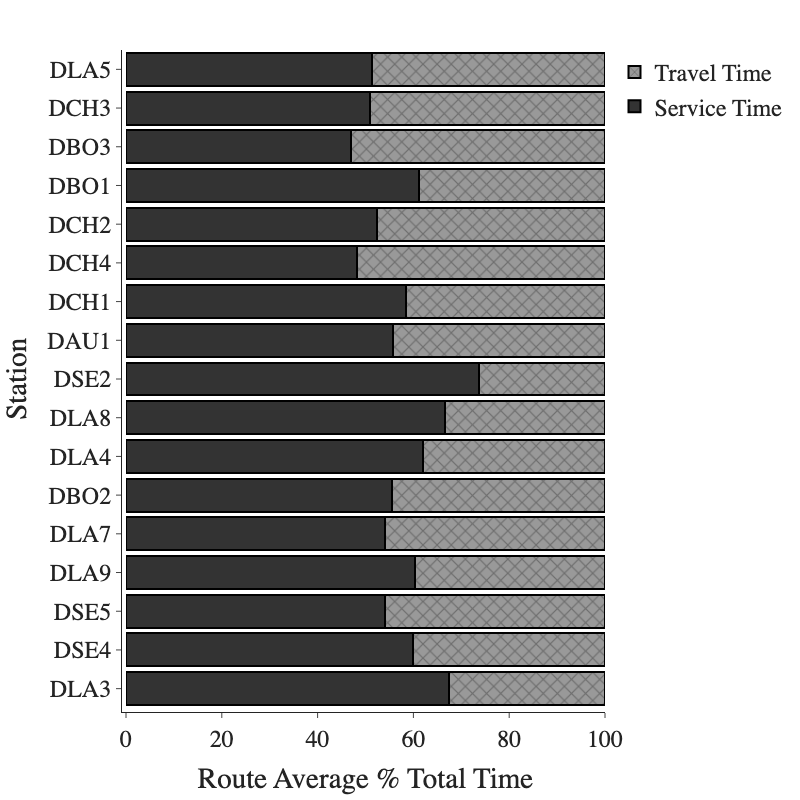
\includegraphics[width=0.5\textwidth]{Images/station_vs_parked_driving.png}
\caption{Comparison of how delivery drivers spend their time vs. the Amazon station from which they depart. The x-axis is normalized as percentage of the average total time. The station code corresponds to an Amazon facility.}
\label{fig:station_vs_parked_driving}
\end{figure}

We plan to explore the role of city zone in predicting service time further in the near-term. Amazon provides their own zone classification that can be leveraged to test our hypothesis that city zones and the characteristics that can be used to describe them contain information about predicted service times. Figure~\ref{fig:city_zones} explores the variance in average service time by zone in Boston, which clearly shows zone average service time is correlated, at least somewhat, with density and proximity to the city center.

\begin{figure}[h!]
\centering
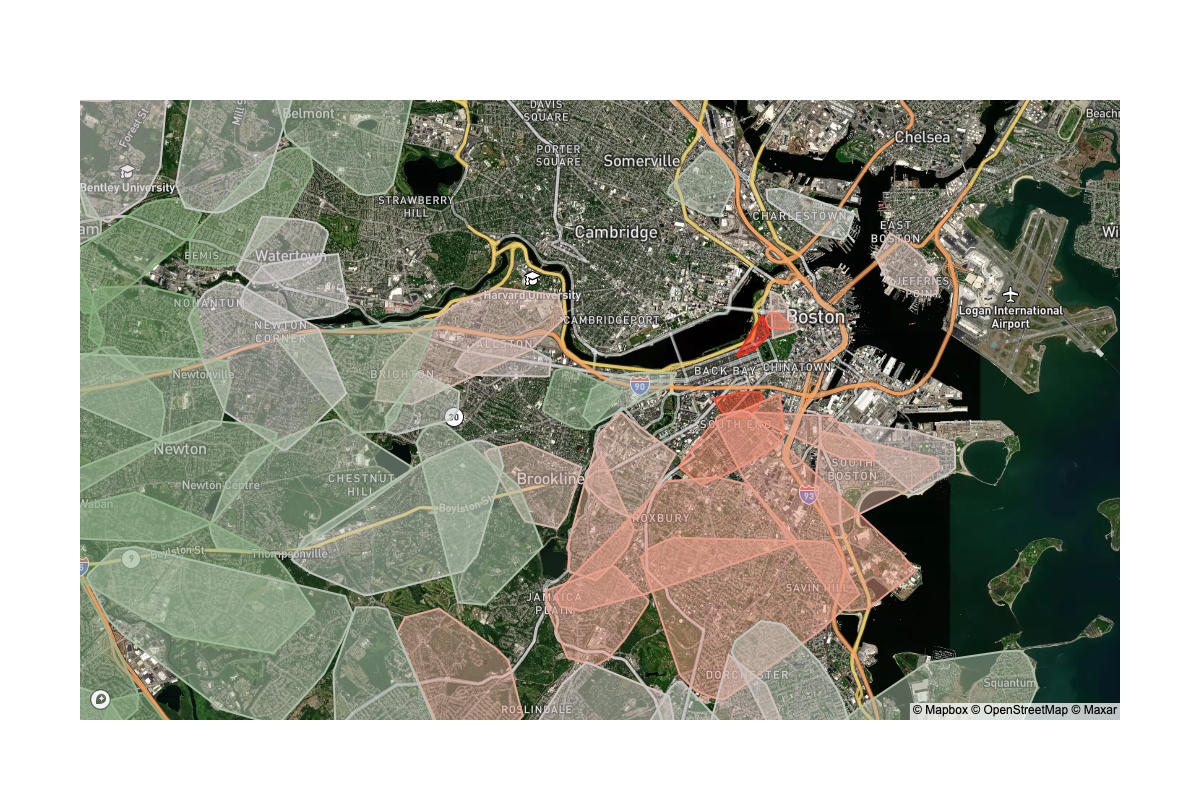
\includegraphics[width=1\textwidth]{Images/zones_n_average_time.png}
\caption{Amazon zones with more than 2 routes are plotted, with green represented zones with lower than average service times and red zones higher than average.}
\label{fig:city_zones}
\end{figure}

% \begin{figure}[h!]
% \centering
% 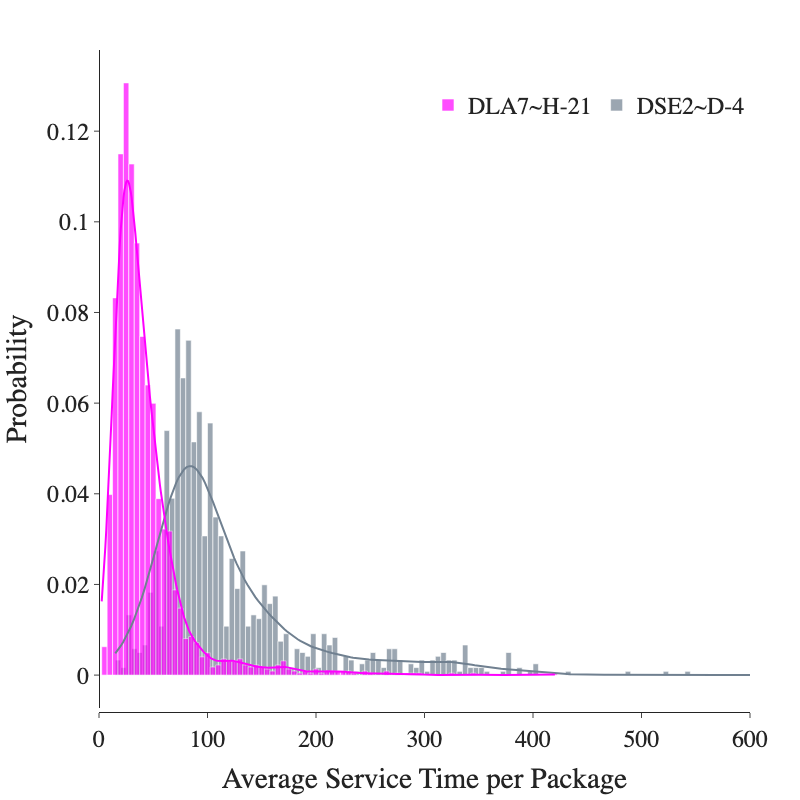
\includegraphics[width=.5\textwidth]{Images/top_and_bottom_zone.png}
% \caption{Probability distribution for the highest and lowest average delivery time zones}
% \label{fig:city_zones}
% \end{figure}

% ------------------------------------------------------
\section{Initial Regression Attempts}

Our goal here is to build an ordinary least squares regression model, and in order to do so we start with analyzing the influence of different parameters on the planned service time provided by Amazon. But before that, we take a look at the distribution of logarithm of min, max and summed planned service times in Fig \ref{fig:service_time_dist} to develop a greater understanding of their behavior. We can see that the distributions are very skewed as we cannot even see the tail after making the $y$-axis logarithmic.

\begin{figure}[h!]
\centering
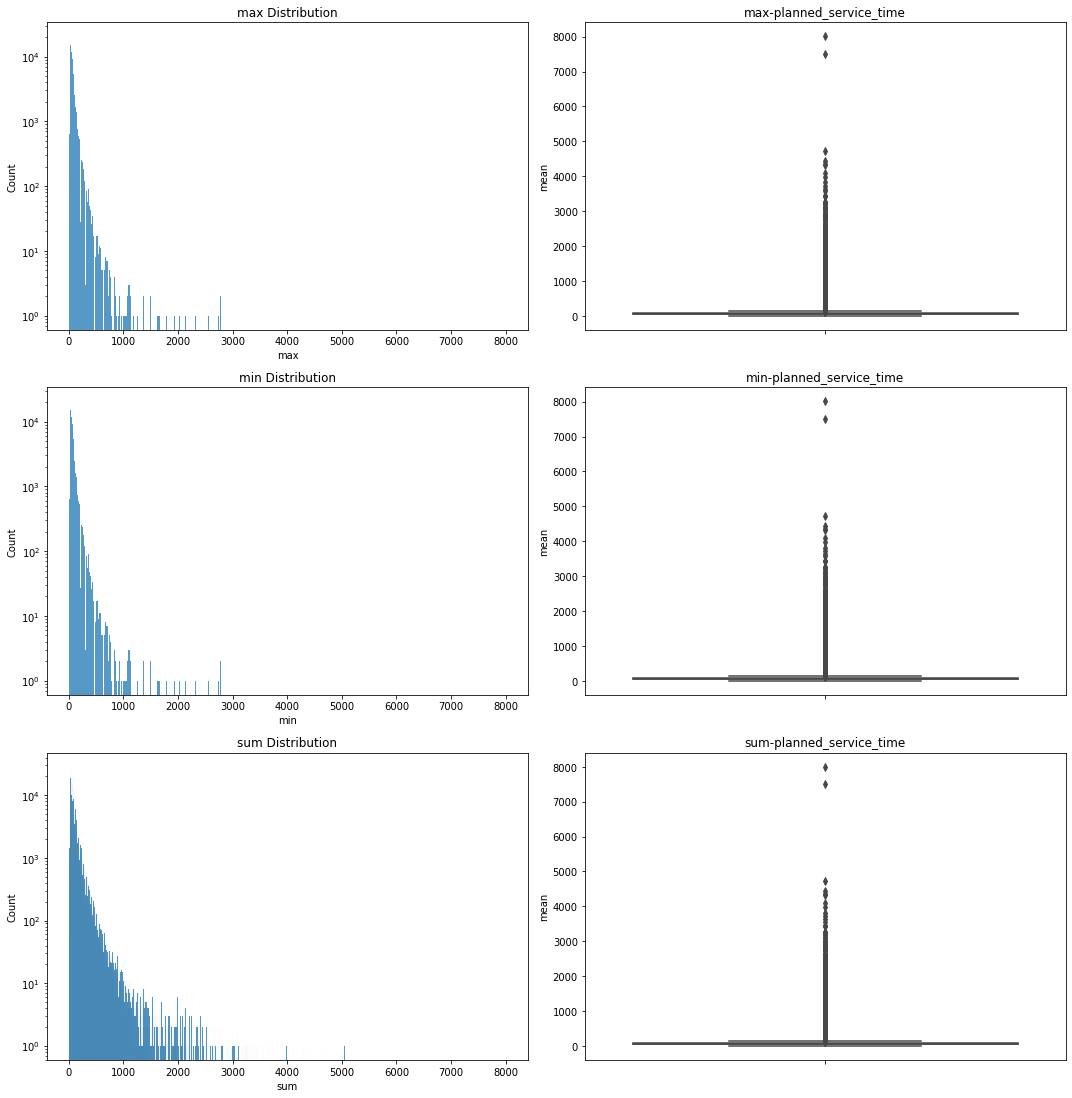
\includegraphics[width=10cm]{Images/service_time_dist.png}
\caption{}
\label{fig:service_time_dist}
\end{figure}


\subsection{Planned Service Times vs Dimension of the package}
Next we look at the scatter plot between \texttt{height}, \texttt{width} and \texttt{volume} of the package and planned service time to see if there a correlation between them. We can clearly see that there is not much correlation between either of these pairs. The coefficient of correlation values we got between the planned service times and width, height, volume are 0.048, 0.74, 0.081 respectively, which indicates almost no correlation.

\begin{figure}[h!]
\centering
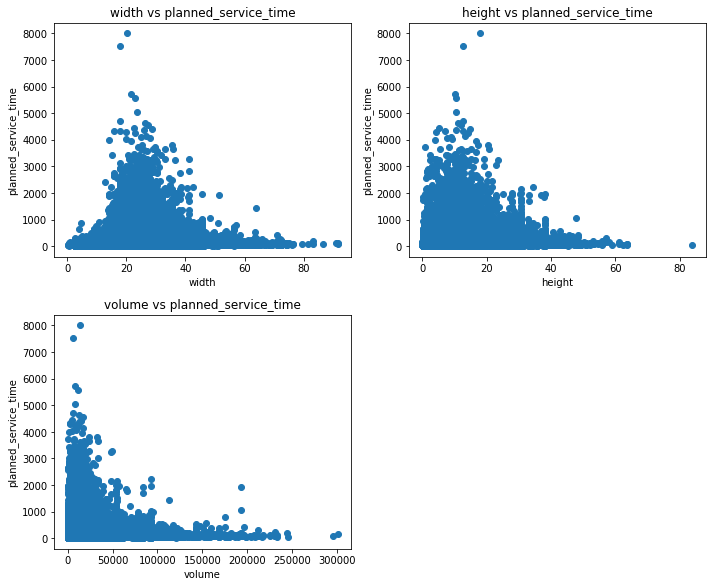
\includegraphics[width=14cm]{Images/dim-scatter.png}
\caption{}
\label{fig:dim-scatter}
\end{figure}


\subsection{Delivery Windows and Status of Delivery}
In Fig \ref{fig:window_and_status}, we try to see whether delivery window (indicated by a binary value \texttt{has\_window}) specified by the customer has any effect on the planned service times proposed by the amazon model. We also plot service times against the \texttt{status} of the delivery. From what can be seen, the only outliers in both the cases belong to the case where delivery was only attempted but never completed. So, we decided to remove these outliers as they were obvious.

\begin{figure}[h!]
\centering
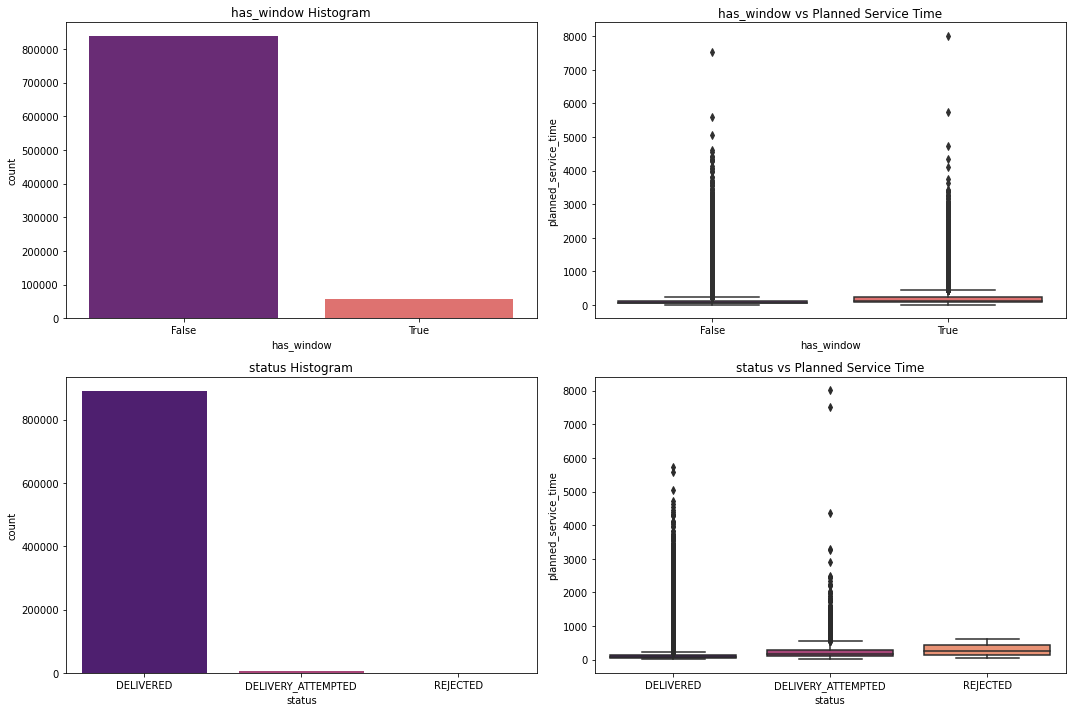
\includegraphics[width=14cm]{Images/window_and_status.png}
\caption{}
\label{fig:window_and_status}
\end{figure}

Figure~\ref{fig:has_window} points to a relationship between a location having a window (\texttt{has\_window}) and also having a longer average service time. Our hypothesis is that customers who specify a windowed delivery time are usually business and apartments complexes. In analysis of small samples, it seems that both businesses and apartment complexes are indicative of longer average service times. Thus, locations with an explicit delivery window have longer predicted service times on average.

\begin{figure}[h!]
\centering
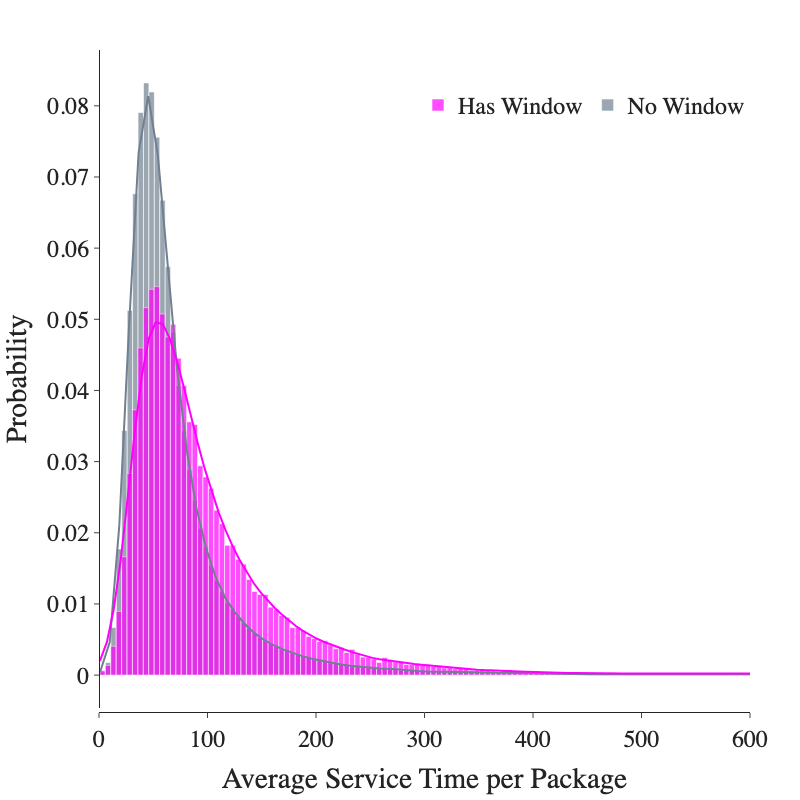
\includegraphics[width=.5\textwidth]{Images/has_vs_no_window.png}
\caption{Probability distribution of average service times for locations with and without specified time windows.}
\label{fig:has_window}
\end{figure}


\subsection{Building Types}

In Fig \ref{fig:building_type}, we consider the type of building information where the delivery was made to understand how do the service times vary in residential versus the business types of buildings. We pulled building type tags using the Microsoft Bing API, by setting a radius around the latitude-longitude pairs given to us for the delivery location, and finally considered only the most relevant tag for buildings in that circular neighbourhood. We can see that there is a bit of variation in the service time depending on the type of building visited, but from the data that we have currently, most of the building types are private residential buildings. Biggest outlier in the data happens for the business type building which makes sense because of the sheer amount and/or volume of deliveries that businesses expect. We define a binary feature value called \texttt{IsPrivateResidence} which takes value \texttt{True} when the building type is residential and \texttt{False}, otherwise.

\begin{figure}
\centering
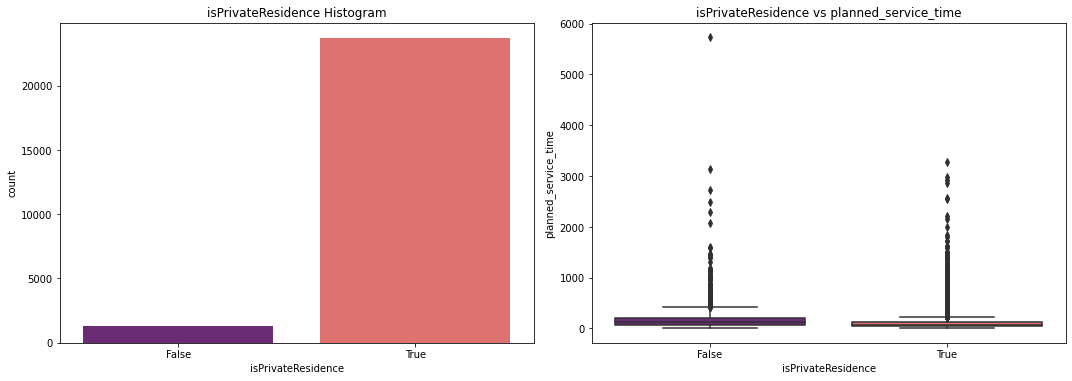
\includegraphics[width=18cm]{Images/building_type.png}
\caption{}
\label{fig:building_type}
\end{figure}

The fact that number of packages might be a really important factor influencing the service time is apparent from their clear correlation that can be seen from Fig \ref{fig:num_packages_scatter} between them. The corresponding correlation coefficient is: $0.58$. Number of packages is referred to as \texttt{num\_packages} in our feature list. While on the other hand, number of stops (\texttt{num\_stops}) doesn't seem to convey much information.


\begin{figure}
\centering
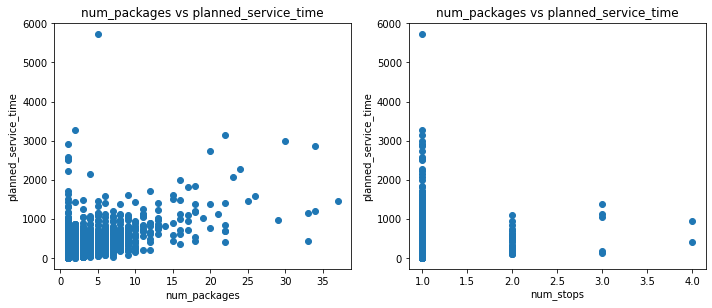
\includegraphics[width=18cm]{Images/num_packages_scatter.png}
\caption{}
\label{fig:num_packages_scatter}
\end{figure}


\subsection{Statistical Tests}

Now, in order to define an OLS regression model we decided to move forward with the following features analyzed so far:
\begin{itemize}
    \item latitude, \texttt{lat}
    \item longitude, \texttt{lng}
    \item height of package, \texttt{height}
    \item width of package,  \texttt{width}
    \item volume of package, \texttt{volume}
    \item number of packages, \texttt{num\_packages}
    \item number of stops, \texttt{num\_stops}
\end{itemize}We discarded all other features as they seemed unrealistic.


After building a regression model using the features defined above we ran Durbin-Watson Test to understand the significance level of these features. As can be seen from Fig \ref{fig:reg1}, features such as \texttt{lat}, \texttt{volume} have p-value more than $0.05$, meaning they are insignificant for our analysis. So, we decided to discard these features and build a model again with just the remaining features.

\begin{figure}
\centering
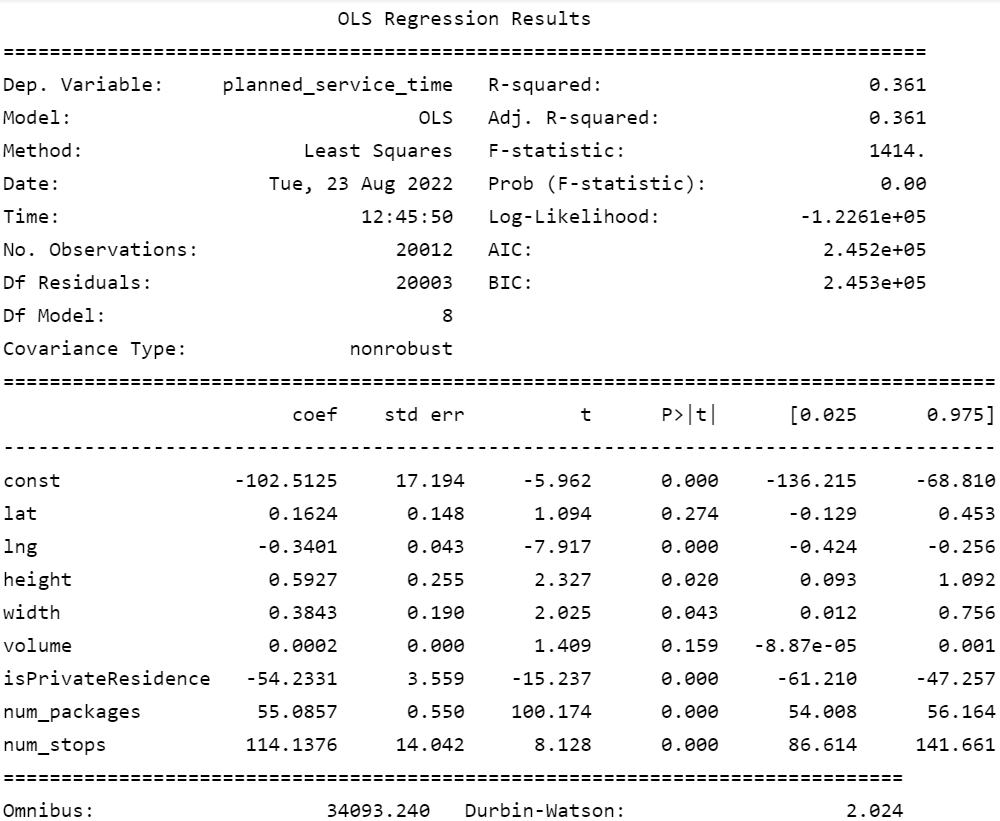
\includegraphics[width=14cm]{Images/reg1.png}
\caption{}
\label{fig:reg1}
\end{figure}


After building the model, we also checked the variance inflation factor (VIF) for all the remaining features, as given in Fig \ref{fig:VIF}, and we see \texttt{height} and \texttt{weight} have the highest VIF relative to other features, so we decided to discard them as well.

\begin{figure}
\centering
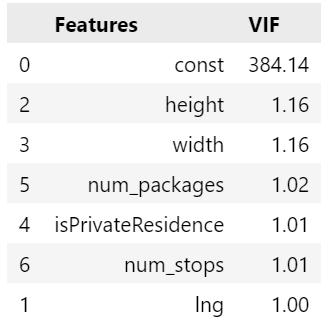
\includegraphics[width=5cm]{Images/VIF.png}
\caption{}
\label{fig:VIF}
\end{figure}

\subsection{Regression Model with selected features}

Finally, we rebuild the model with all the left out features so far and  redoing the Durbin-Watson test, as shown in Fig \ref{fig:reg2}, confirms that none-of the remaining features are insignificant in terms of their p-value. Fig \ref{fig:Error} shows the distribution for the training error we got, which is a skewed Gaussian distribution as expected.
\begin{figure}
\centering
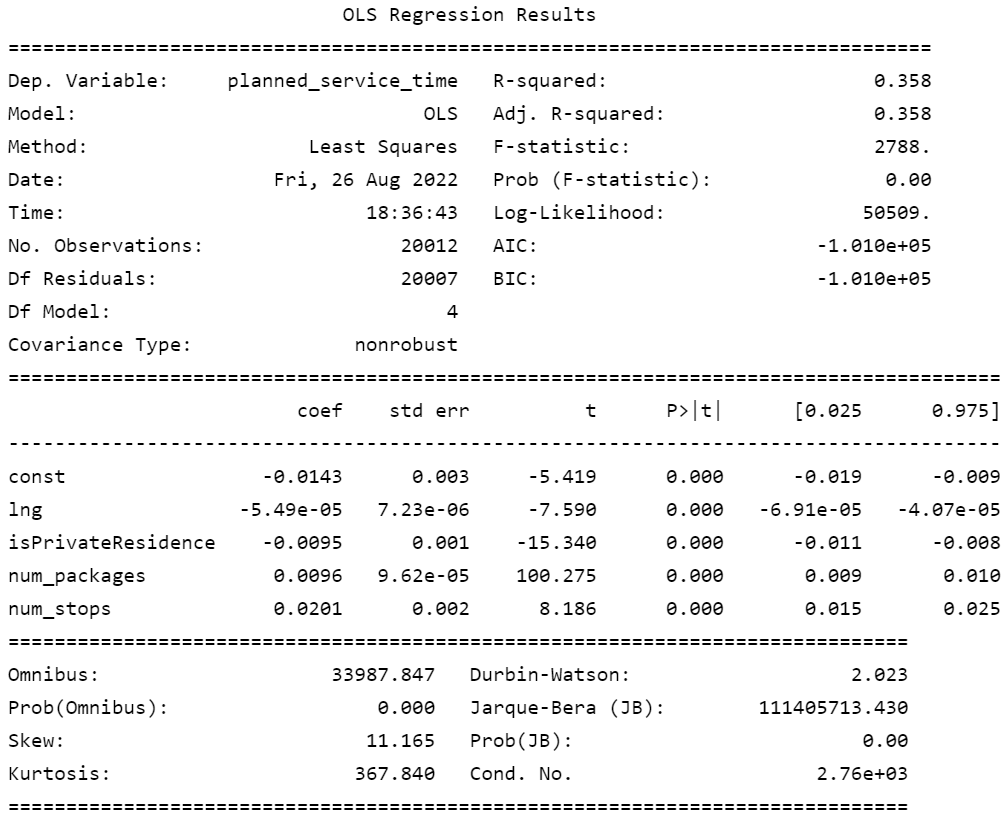
\includegraphics[width=14cm]{Images/reg2.png}
\caption{}
\label{fig:reg2}
\end{figure}

\begin{figure}
\centering
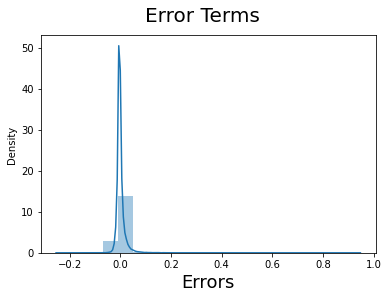
\includegraphics[width=12cm]{Images/Error.png}
\caption{}
\label{fig:Error}
\end{figure}

Finally, Fig \ref{fig:test_pred} indicates the scatter plot between the predicted $y$-values for the test dataset and the actual $y$-values. Ideally, it should been a straight line but the clear deviation from straight line indicates missing data as we already utilized all the possible given features. \unsure{if this narrative is correct?}

\begin{figure}
\centering
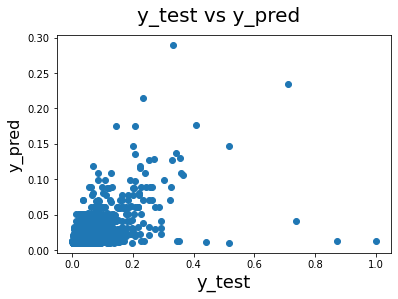
\includegraphics[width=12cm]{Images/test_pred.png}
\caption{}
\label{fig:test_pred}
\end{figure}


% -------------References-----------------
\bibliographystyle{plain}
\bibliography{references}


\end{document}